\section{Online profiling}
\label{sec:online}

Our first technique, called online profiling, periodically re-profiles 
the resource-accuracy tradeoffs of each knob and reduces the 
re-profiling costs by updating one knob at a time while fixing the 
values on other knobs.
By treating the knobs separately, we can reduce the re-profiling cost 
from $O(n^k)$, an exhaustive search (Policy~2) in $k$ knobs each having 
$n$ values, to $O(n\cdot k)$.


\mypara{Independence among knobs}
The insight underlying how Policy~3 cuts profiling cost is that, for
each knob, the relationship between its value and inference accuracy is 
independent to the setting on other knobs. 
That is, for instance, if 5fps is the least frame rate to get an F1 score
of 0.8 when the frame size is 960p, then 5fps will be the least frame rate 
to attain an F1 score of 0.8 when the frame size is 480p.
The intuition behind the independence between knobs is that the impact of
these knobs on accuracy is determined by {\em orthogonal} factors. 
For instance, in pipeline $A$, the frame rate concerns the object moving
speed, image sizes concerns the number of pixels to cover each object of
interest, and the object detection model depends on whether the shape of
an object can be expressed by the extracted features.
This allows us to profile knobs separately, and safely ignore the 
combinational effects between knobs.

\jc{add a table of notation here}

\begin{algorithm}[t!]
\small
	\DontPrintSemicolon
    \SetKwFunction{Overall}{ConfigAdaptation}
    \SetKwFunction{ProfilingUnit}{OnlineProfiling}
    \SetKwProg{Fn}{Function}{:}{}
	\KwIn{$n$ video feed $M_1,\dots,M_n$, the accuracy threshold $\alpha$, and all possible configurations $C$, each being a combination of values on $k$ knobs, where $V_k$ and $v_k^*$ are the values of knob $k$ and its most expensive value.}
	\KwOut{Configuration $\hat{c}_{M_i,T_j}$ for video $M_i$ in time window $T_j$.}
% 	\Fn{\Overall{$\{M_1,\dots,M_n\}, C, \alpha$}}{
%         \ForEach{$j$-th $T$-second time window $T_j$}{
%     	    \ForEach{$M_i$}{
%         	    $X_{i,j}\leftarrow I(M_i,t_j)$\\
%         	    $\hat{c_{M_i,T_j}}\leftarrow \ProfilingUnit(X_{i,j},C,\alpha)$\\
%         	}
%     	}
%     	\Return{$\hat{c}_{M_i,T_j}$ for all $M_i$ and $T_j$}
% 	}
    \Fn{\ProfilingUnit{$X, C, \alpha$}}{
        $c^{default}=(v_1^{default},\dots,v_m^{default})$\\
        \tcc{\small{Optimize one knob at a time}}
        \ForEach{Knob $k$}{
            $R_{min}\leftarrow\infty$; $A_{best}\leftarrow 1$\\
            \ForEach{$v_k\in V_k$}{
                \tcc{\small{Change only knob $k$ to $v_k$}}
                $c(v_k)\leftarrow Replace(c^{default},k,v_k)$\\
                $c(v_k^*)\leftarrow Replace(c^{default},k,v_k^*)$\\
                $A\leftarrow F(X,c(v_k),c(v_k^*))$\\
                \tcc{\small{Set knob $k$ to $v$, if $v$ is cheaper and is accurate enough}}
                \If{$R(c(v_k)) < R_{min}$ \textrm{\bf and} $A \geq \alpha$}{
                    $\hat{v_k}\leftarrow v$; $R_{min}\leftarrow R(c(v_k))$; $A_{best}\leftarrow A$\\
                }
            }
            \tcc{\small{Update the accuracy threshold}}
            $\alpha=\frac{\alpha}{A_{best}}$
        }
        \Return{$\hat{c}\leftarrow(\hat{v_1},\dots,\hat{v_n})$}
    }
	\caption{Online Profiling.}
	\label{alg:policy3}
\end{algorithm}

\mypara{Profiling knobs separately}
Policy~\ref{alg:policy3} describes online profiling in action. 
Let $Replace(C,k,v)$ denote the result of setting knob $k$
of $C$ with $v$, and $F(X,c,c^*)=\frac{1}{|X|}\sum_{x\in X}f(x,c,c^*)$ denote
the average F1 score of $c$ with respect to $c^*$ over a set of frames $X$.
For every $T$ seconds, it re-profiles and updates the configurations
on the frames in the first $t$ seconds.
For each knob $k$, it tries all of its possible values while fixing 
other knobs to their default values $C(v_k)$, and calculate the accuracy 
with respect to setting knob $k$ to its most expensive values as the golden
configuration $C(v_k^*)$ (line~5-7). 
This allow us to identify the ``sweet spot'' value of knob $k$ that has 
least resource consumption while achieving enough accuracy 
(line~8-9).
Finally, since the accuracy degradation of individual knobs will 
be accrued when combining them together, we increase the accuracy 
threshold after each knob is updated (line~10).
% Given a configuration $C$, configuration 
% $C'=C\setminus\{v_k\}\cup \{v_k^*\}$ has the same values to $C$ except for the $k$-th knob, on which $C$ has $v_k$ and $C^*$ has $v_k^*$.
There are two more details in online profiling.
First, for some knobs (e.g., frame rate, minimal area size), a lower value
has no profiling cost, if a higher value has been profiled, because the 
output of the lower value can be extrapolated from the output of a higher 
values (e.g., for frame rate, it means simply ignoring frames in the 
higher frame rate output).
Second, Policy~3 depends on the default values, though different settings
of default values only yield marginal performance 
difference.~\footnote{We notice that such independence would be weakened in 
extreme cases; e.g., it is hard to profile the accuracy of different
frame rates, under too small an image size, as no \nn would detect any
objects. So when profiling a certain knob, other knobs are not set to
such extreme values.}


% by ignoring the interaction between 
% knobs. 
% The insight behind this idea is that in video analytics, the 
% resource-accuracy tradeoffs of configurations depend on mostly independent
% aspects of videos, so the sweet-spot of the resource-accuracy tradeoff of
% a certain knob is often independent to the value of other knobs.
% For instance, the best frame sampling rate that strikes a balance between accuracy 
% and resource depends on the speed of objects, while the best image size depends
% on the size of the objects of interest. 


Figure~\ref{fig:policy3} shows the improvement by online profiling 
on two video clips.
We can see that the configuration picked by online profiling achieves 
similar resource-accuracy tradeoffs to Policy~2, and still much better 
than Policy~1. 
In the meantime, the profiling cost is significantly reduced relative to
Policy~2. \jc{TODO}
Nonetheless, most of the gains of online configuration adaptation is 
negated by the profiling cost.

% Formally, this can be described as following. 
% Given two configurations $C_1$ and $C_2$ that share the same value $v$ 
% on certain knob, suppose that the most expensive value of the knob is $v^*$, and
% let $F(x,C,C\setminus\{v\}\cup \{v^*\})$ denote 
% the accuracy of configuration $C$ 
% on frame $x$, if substituting $v$ by $v^*$ in $C$ is the golden configuration.
% \begin{align*}
%     F(x,C_1,C_1\setminus\{v\}\cup \{v^*\})=
%     F(x,C_2,C_2\setminus\{v\}\cup \{v^*\})
% \end{align*}

% This is consistent with our empirical results.
% See Figure~\ref{fig:potential}

% \begin{figure}
%     \centering
%     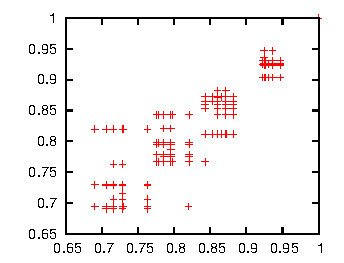
\includegraphics[width=0.25\textwidth]{figures/Profile_Sampling.pdf}
%     \caption{X and Y axises are $F(x,C_1,C_1\setminus\{v\}\cup \{v^*\})$ and $F(x,C_2,C_2\setminus\{v\}\cup \{v^*\})$, respectively. Accuracy of the frame sampling rate is conditionally independent to 
%     the values of other configuration knobs.}
%     \label{fig:}
% \end{figure}

\begin{figure}
    \centering
    \hspace{-0.5cm}
    \subfloat[Video clip \#1]
    {
        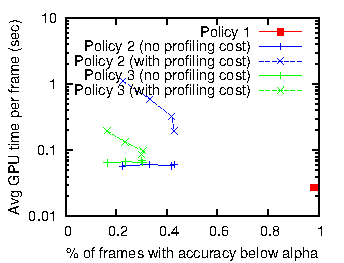
\includegraphics[width=0.25\textwidth]{figures/Bellevue_116th_NE12th_accThresh_80p_Comparison_Policy123.pdf}
        \label{subfig:1}
    }
    \subfloat[Video clip \#2]
    {
        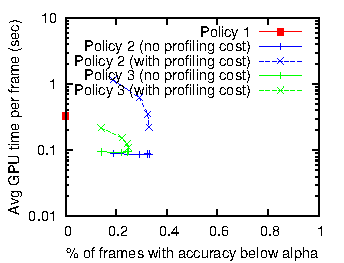
\includegraphics[width=0.25\textwidth]{figures/Bellevue_150th_Eastgate_accThresh_80p_Comparison_Policy123.pdf}
        \label{subfig:2}
    }
    \caption{}
    \label{fig:policy3}
\end{figure}

% \begin{policy}[Periodic Per-knob Search]
% See Algorithm~\ref{alg:policy3}
% \end{policy}
